\documentclass{article}      % Specifies the document class

% -------------------- Packages --------------------
\usepackage{amsmath}
\usepackage{amssymb}
\usepackage[noend]{algpseudocode}
\usepackage{algorithm}
\usepackage{graphicx}
\usepackage{float}
\usepackage{fontawesome5}
\usepackage{listings}

\lstset{language=Python,keywordstyle={\bfseries \color{blue}}}
\NewDocumentCommand{\codeword}{v}{%
    \texttt{\textcolor[HTML]{5c5c65}{#1}}%
}


\usepackage{hyperref}
\hypersetup{
    colorlinks=true,
    linkcolor=blue,
    filecolor=magenta,      
    urlcolor=cyan,
    pdftitle={Overleaf Example},
    pdfpagemode=FullScreen,
    }

\urlstyle{same}

\usepackage{bookmark}
\hypersetup{hidelinks} %enlève les cadres rouges autour des hyperliens


% ---------- PSEUDO CODE : hack to remove indent ----------
% https://tex.stackexchange.com/questions/354564/how-to-remove-leading-indentation-from-algorithm
\usepackage{xpatch}
\makeatletter
\xpatchcmd{\algorithmic}
  {\ALG@tlm\z@}{\leftmargin\z@\ALG@tlm\z@}
  {}{}
\makeatother

\usepackage{xcolor}
\usepackage[framemethod=tikz]{mdframed}
\usepackage{tikzpagenodes}
\usetikzlibrary{calc}


% -------------------- Couleurs --------------------
\definecolor{definition}{HTML}{2f80ed}
\definecolor{definition-bg}{HTML}{e0ecfd}

\definecolor{danger}{HTML}{e6505f}
\definecolor{danger-bg}{HTML}{fce5e7}

\definecolor{exogris}{gray}{0.4}



% -------------------- Code --------------------
\definecolor{codegreen}{rgb}{0,0.6,0}
\definecolor{codegray}{rgb}{0.5,0.5,0.5}
\definecolor{codepurple}{rgb}{0.58,0,0.82}
\definecolor{backcolour}{rgb}{0.95,0.95,0.92}

\lstdefinestyle{code-style}{
    backgroundcolor=\color{backcolour},   
    commentstyle=\color{codegreen},
    keywordstyle=\color{magenta},
    numberstyle=\tiny\color{codegray},
    stringstyle=\color{codepurple},
    basicstyle=\ttfamily\footnotesize,
    breakatwhitespace=false,         
    breaklines=true,                 
    captionpos=b,                    
    keepspaces=true,                 
    numbers=left,                    
    numbersep=5pt,
    showspaces=false,                
    showstringspaces=false,
    showtabs=false,                  
    tabsize=2
}

% -------------------- Styles --------------------
\mdfdefinestyle{definition-style}{%
  innertopmargin=10px,
  innerbottommargin=10px,
  linecolor=definition,
  backgroundcolor=definition-bg,
  roundcorner=4px
}
\newmdenv[style=definition-style]{definition}

\mdfdefinestyle{danger-style}{%
  innertopmargin=10px,
  innerbottommargin=10px,
  linecolor=danger,
  backgroundcolor=danger-bg,
  roundcorner=4px
}
\newmdenv[style=danger-style]{danger}


% -------------------- Document --------------------
\title{Théorie des Graphes\\\Large{Projet noté}}
\author{MADANI Abdenour\\TRIOLET Hugo}
\date{Licence 3\\2021 - 2022}
\begin{document}
\normalsize
\maketitle

\renewcommand*\contentsname{Table des matières}
\tableofcontents
\newpage



\section{Introduction}
\subsection{Objectifs}
Les objectifs de ce TPs sont :
\begin{itemize}
  \item Orienter un graphe non-orienté en un graphe fortement connexe,
  \item Décomposer en graphe en chaînes (selon Schmidt$^\text{\cite{schmidt}}$),
  \item Établir si un graphe est 2-connexe ou 2-arête,
  \item Calculer les composantes 2-connexes et 2-arêtes-connexes sinon.
\end{itemize}

On utilisera pour ceci \textbf{SageMath} (bibliothèque de fonctions pour Python).



\subsection{Définitions}
\begin{definition}
{ \scriptsize \textcolor{definition}{\faIcon{graduation-cap} \textbf{DÉFINITION}}}
\vspace{3px}
\\ \underline{\textbf{Pont}}
\vspace{2.5px}
\\ Arête dont la suppression augmente le nombre de composantes connexes du graphe restant.%
\\ \textit{(aussi appelé arête déconnectante)}
\end{definition}

\begin{definition}
{ \scriptsize \textcolor{definition}{\faIcon{graduation-cap} \textbf{DÉFINITION}}}
\vspace{3px}
\\ \underline{\textbf{Sommet d'articulation}}
\vspace{2.5px}
\\ Sommet dont la suppression augmente le nombre de composantes connexes du graphe restant.%
\\ \textit{(aussi appelé sommet déconnectant ou noeud d'articulation)}
\end{definition}

\begin{definition}
{ \scriptsize \textcolor{definition}{\faIcon{graduation-cap} \textbf{DÉFINITION}}}
\vspace{3px}
\\ \underline{\textbf{2-connexité (\textit{2-sommet-connexité})}}
\vspace{2.5px}
\\ Un graphe est dit 2-connexe s'il n'admet pas de sommet d'articulation.
\end{definition}

\begin{definition}
{ \scriptsize \textcolor{definition}{\faIcon{graduation-cap} \textbf{DÉFINITION}}}
\vspace{3px}
\\ \underline{\textbf{2-arête-connexité}}
\vspace{2.5px}
\\ Un graphe est dit 2-arête-connexe s'il n'admet pas de pont.
\end{definition}

\begin{definition}
{ \scriptsize \textcolor{definition}{\faIcon{graduation-cap} \textbf{DÉFINITION}}}
\vspace{3px}
\\ \underline{\textbf{Depth-First Search (DFS)}}
\vspace{2.5px}
\\ Parcours en profondeur d'un graphe.
\end{definition}

\begin{definition}
{ \scriptsize \textcolor{definition}{\faIcon{graduation-cap} \textbf{DÉFINITION}}}
\vspace{3px}
\\ \underline{\textbf{Depth-First Index (DFI)$^\text{\cite{schmidt}}$}}
\vspace{2.5px}
\\ Date à laquelle le DFS a \textbf{débuté} sur un noeud.
\end{definition}

\begin{definition}
{ \scriptsize \textcolor{definition}{\faIcon{graduation-cap} \textbf{DÉFINITION}}}
\vspace{3px}
\\ \underline{\textbf{Graphe sous-jacent}}
\vspace{2.5px}
\\ Pour un graphe orienté, le graphe sous-jacent correspond au graphe avec les mêmes noeuds, mais dont les arêtes ne sont plus orientées. (le graphe sous-jacent est donc non-orienté)
\end{definition}

\subsection{Résumé de notre approche}
On implémente la décomposition en chaînes$^\text{\cite{schmidt}}$.
\\Celle-ci nous permet d'obtenir tous les ponts, ainsi que tous les sommets d'articulation du graphe.
\\On en déduit ensuite si le graphe est 2-connexe, 2-arête-connexe, ou aucun des deux, grâce à l'Algorithme 1 de Schmidt$^\text{\cite{schmidt}}$.
\\On calcule ensuite les composantes 2-connexes et 2-arêtes-connexes.
\\\\Vis-à-vis du code, nous l'avons documenté à l'aide de la \textit{docstring} de Python, les fonctions se comprennent donc naturellement grâce à celle-ci.
%


\section{Exercices}
\subsection{Exercice 1}
\textit{\textcolor{exogris}{
Dans une premier temps il est demandé d’implémenter les algorithmes de calcul de 2-connexité dû à Schmidt$^\text{\cite{schmidt}}$.
\\(1) Calculer les composantes 2-connexes d’un graphe.
\\(2) Calculer les composantes 2-arêtes-connexes d’un graphe.
}}
\\On commence par effectuer la décomposition en chaînes.
\\\textbf{Pour obtenir les composantes 2-connexes :}
\\On prend le graphe original, 
\\Ensuite, on enlève les noeuds restants de degré 0.
%
%
\\\\\textbf{Pour obtenir les composantes 2-arêtes-connexes :}
\\On prend le graphe original, on supprime ses ponts.
\\Ensuite, on enlève les noeuds restants de degré 0.
\\Voir fonction \codeword{calcule_comp_2_arete_connexe}.
%



\subsection{Exercice 2}
\textit{\textcolor{exogris}{
Trouvez un orientation en un graphe fortement connexe$^\text{\cite{schmidt}}$ ou trouvez une arête déconnectante.
}}
\\On effectue un DFS pour orienter toutes les arêtes, tel que décrit par Schmidt\textit{Figure 1b}$^\text{\cite{schmidt}}$.
\\On oriente les arcs de parenté du fils vers le père, et les arcs arrières du père vers le fils.
\\D'après le théorème de Robbins$^\text{\cite{robbins}}$, le graphe orienté obtenu sera fortement connexe si et seulement si celui-ci était 2-arête-connexe.
\\\\Au sein de notre fonction \codeword{parcours_graphe()}, nous avons une sous-fonction \codeword{parcours()} qui est une fonction récursive de DFS.
\\Si jamais le graphe n'est pas connexe, nous faisons appel à la fonction \codeword{lance_parcours()} qui lance un DFS sur chaque sommet non-visité.
\\Durant la fonction \codeword{parcours()}, nous allons créer un nouveau graphe qui contiendra, en \textcolor[HTML]{333333}{gris foncé}, \textbf{l'arbre de parcours en profondeur}, et en \textcolor[HTML]{a0a0a0}{gris clair} tous les arcs arrières.
\begin{danger}
{ \scriptsize \textcolor{danger}{\faIcon{exclamation-triangle} \textbf{ATTENTION}}}
\vspace{3px}
\\ Ce graphe est appelé \codeword{arbre_parcours} dans le code (bien qu'il contienne les arcs arrière).
\end{danger}

\begin{figure}[H]
    \centering
     \scalebox{.35}{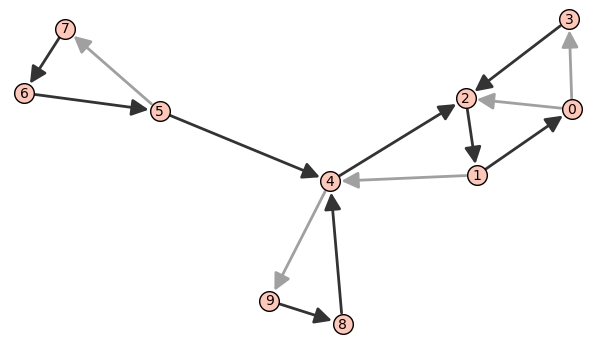
\includegraphics{graphe-oriente-gris.png}}
    \\\codeword{arbre_parcours}
\end{figure}

Pour plus de commodités, nous créons aussi deux graphes à part contenant chacun soit uniquement l'arbre de parcours, soit uniquement les arrières : appelés respectivement \codeword{arbre_parcours_uniquement} et \codeword{arriere}.

\begin{figure}[H]
    \centering
     \scalebox{.35}{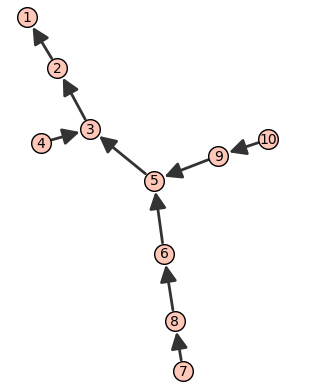
\includegraphics{arbre_parcours_uniquement.png}}
    \\\codeword{arbre_parcours_uniquement}
\end{figure}

\begin{figure}[H]
    \centering
     \scalebox{.35}{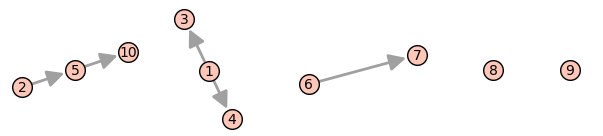
\includegraphics{arriere.png}}
    \\\codeword{arriere}
\end{figure}

Le graphe \codeword{arbre_parcours} est donc une orientation en graphe fortement connexe si et seulement si la variable \codeword{deux_arete_connexe} renvoyée par la fonction vaut \codeword{True}.
\\Si \codeword{deux_arete_connexe} vaut \codeword{False}, alors il suffit de regarder la variable \codeword{ponts} renvoyée par la fonction (ou \codeword{graphe_ponts.edges()}).



\subsection{Exercice 3}
\textit{\textcolor{exogris}{
Montrez qu’un graphe est fortement connexe$^\text{\cite{schmidt}}$ si et seulement si chaque arc est présent dans au moins un circuit de G.
}}
\\todo



\subsection{Exercice 4}
\textit{\textcolor{exogris}{
Prouvez ou infirmez l’affirmation suivante :
\\Un graphe est fortement connexe si et seulement si son graphe sous-jacent est 2-arête connexe.
}}
\\Voici un exemple qui infirme la proposition.
Soit ce graphe non-orienté :

\begin{figure}[H]
    \centering
     \scalebox{.35}{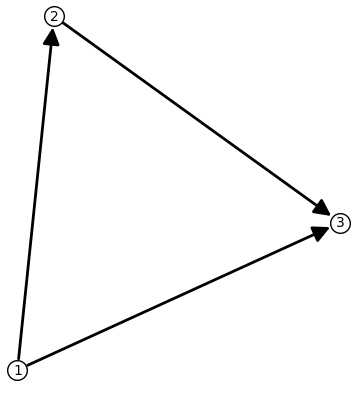
\includegraphics{exo4-g2.png}}
    \\Un graphe orienté non fortement connexe
\end{figure}

Celui-ci n'est pas fortement connexe, car on ne peut pas accéder à 1 à partir de 3 par exemple.
Or voici son graphe sous-jacent :
\begin{figure}[H]
    \centering
     \scalebox{.35}{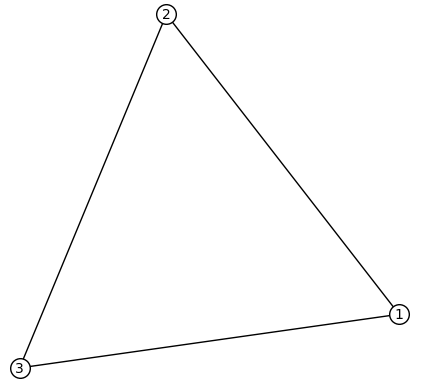
\includegraphics{exo4-g1.png}}
    \\Son graphe sous-jacent
\end{figure}
Celui-ci est bien 2-arête-connexe, pourtant le graphe original n'était pas fortement connexe, cela conclut la preuve.



\section{Exemples d'utilisation du code}
\subsection{Comment utiliser le code}
Il faut évidemment disposer de SageMath pour exécuter le code.
Par exemple, en l'installant sur le site officiel, et en l'exécutant dans un NoteBook tel que Jupyter.

\begin{lstlisting}[style=code-style]
k4 = graphs.CompleteGraph(4)
k4, pont_k4, c2ac, sommet_art, c2sc = parcours_graphe(k4)
print('hello')
\end{lstlisting}

\subsection{Graphes testés}
todo



\section{Références}
\begin{thebibliography}{9}
\bibitem{robbins}
Herbert Robbins, \textit{A theorem on graphs, with an application to a problem on traffic control}, American Mathematical Monthly 46, 281–283.

\bibitem{schmidt}
Jens M. Schmidt, \href{https://arxiv.org/ftp/arxiv/papers/1209/1209.0700.pdf}{\underline{\textit{A Simple Test on 2-Vertex- and 2-Edge-Connectivity}}},
\\Inf. Process. Lett. \textbf{113} (2013), no. 7, 241–244.
\end{thebibliography}



\section{Annexe}
\subsection{Code SageMath}

\end{document}
